\chapter{Data and Event Log}
\label{cap:datos}

This chapter describes the data of the work and the event log built from them. It presents the source database and the tables used, with an example of their content. It then describes the case attributes and the selected population. Next, it presents the reference model of the process and the construction of the event log. Finally, it defines the candidate outcome labels, analyzes the relation between the planned destination and the actual ICU admission, lists the sources of information leakage and computes the entropy of the process. All of this conditions the experiments of Chapter~\ref{cap:implementacion}.

\section{The \code{ftr\_cige\_v01} Database}
\label{sec:bd}

The data come from a research project on FTR in inpatients. In that project, the two research groups of UJI introduced in Section~\ref{sec:contexto} collaborate: GIANT, which contributes the ML and PM expertise, and GIENF, which contributes the clinical and nursing expertise. The data are real: they are the records of the \emph{Hospital Universitari de La Plana} (Vila-real, Castell\'o) for the adult patients hospitalized between March 2023 and April 2024, extracted from its hospital information system and anonymized before being handed over to the research groups. The result is the \code{ftr\_cige\_v01} database, hosted on a PostgreSQL server at UJI. The copy used in this work was exported in March 2026.

The database has 20 tables. The central concept is the \textbf{episode}: a hospitalization of one patient, from the admission date to the discharge date, identified by an anonymized episode code. A patient may have several episodes in the period, and therefore the patient code is a different, also anonymized, identifier. Every other table refers to the episode through its code. The tables can be grouped as follows.

\begin{itemize}[leftmargin=*]
  \item \textbf{Hospitalization}. The main table \code{ftr\_hosp} (9,304 rows, one per episode) and its satellite tables: inter-service consultations (\code{ftr\_hosp\_interconsultas}, 6,704 rows), surgical interventions (\code{ftr\_hosp\_int\_quirurgicas}, 2,319), transfers between beds and units (\code{ftr\_hosp\_traslados}, 1,993) and ICD-10 coding at discharge (\code{ftr\_hosp\_codificacion}, 79,417).
  \item \textbf{Emergency care}. The visit to the emergency department that precedes an urgent admission (\code{ftr\_hosp\_urg}), with its vital signs, coding and laboratory tests (four tables).
  \item \textbf{Monitoring during the stay}. Vital-sign readings (\code{ftr\_hosp\_ctes}, 621,752 rows), laboratory requests and results (\code{ftr\_hosp\_lab} and \code{ftr\_hosp\_lab\_resultados}, 459,354 results) and nursing assessments (\code{ftr\_hosp\_valenf}, 16,942).
  \item \textbf{Catalogs}. Code tables with the description of each code: services (\code{codigo\_servicio}), discharge reasons (\code{motivo\_alta\_pk}), anesthesia types (\code{tipo\_anestesia\_pk}), postoperative destinations (\code{destinos\_postoperatorio\_quirofano}) and laboratory parameters.
\end{itemize}

\subsection{From the Whole Database to the Tables Used}
\label{sec:historia_tablas}

The tables used in the final event log were not fixed from the start. They were selected in three steps, which also define the three versions of the event log mentioned in this report.

\begin{enumerate}[leftmargin=*]
  \item \textbf{Event log version 1} (preliminary version). A first event log was built from all 20 tables, with the whole hospitalization process and all the 9,304 episodes as cases. Each clinical act was an event: every vital-sign reading, every laboratory request and result, every nursing assessment. The purpose was to become familiar with the case study: which acts are recorded, with which timestamps and with which quality. The result was an event log of about 516,000 events, with a median of 42 events per case and 9,063 distinct variants among 9,304 cases. Almost every case was unique. Such an event log cannot be represented by a process model of reasonable size, and the monitoring tables (vital signs and laboratory) contribute many events but no decision of the process.
  \item \textbf{Event log version 2 (scope reduction)}. The work was limited to one branch of the process, the elective surgical admission (Section~\ref{sec:poblacion}), and to the acts that define its course: admission, consultations, surgery, transfers and discharge. These acts live in four tables, the hospitalization, consultations, interventions and transfers tables, which were enough to model the hospitalization. The coding table and the catalogs were kept only for the case attributes and the descriptions. The emergency care, vital signs, laboratory and nursing assessment tables were left outside the scope. This gave \textbf{event log version 2}, with 10 activities.
  \item \textbf{Event log version 3} (final version). The postoperative destination recorded in the surgical table became an activity of its own (Section~\ref{sec:construccion}). This is the version used in the whole report. When the report compares `version 2' with `version 3', it refers to these two event logs, which differ only in the destination activities.
\end{enumerate}

Table~\ref{tab:tablas} summarizes the tables used in the final event log and the use given to each one.

\begin{table}[H]
\centering
\caption{Tables of \code{ftr\_cige\_v01} used in the event log.}
\label{tab:tablas}
\small
\begin{tabular}{L{4.7cm}L{8.9cm}}
\toprule
Table & Content and use \\
\midrule
\code{ftr\_hosp} & Hospitalization episode: anonymized patient and episode, age and sex, admission and discharge dates, admission type, process type, admitting and discharge services, discharge reason, admission diagnosis, date of death, readmission within 7 days, beds and palliative care. Main table; it defines the case. \\
\code{ftr\_hosp\_interconsultas} & Consultations requested during the episode: date, priority, requesting service, target service and text of the request. \\
\code{ftr\_hosp\_int\_quirurgicas} & Surgical interventions: start and end, service, type, diagnosis, procedure, anesthesia, planned postoperative destination (\code{codigo\_destino}), approach and category. \\
\code{ftr\_hosp\_traslados} & Actual movements of the patient between beds and units within the hospital: bed, service, start and end dates and the ordinal of the movement. \\
\code{ftr\_hosp\_codificacion} & ICD-10 diagnostic coding of the episode, performed at discharge, with the order of each diagnosis. Only for the case attributes. \\
Catalogs & \code{codigo\_servicio}, \code{motivo\_alta\_pk}, \code{tipo\_anestesia\_pk} and \code{destinos\_postoperatorio\_quirofano}, for the descriptions of the codes. \\
\bottomrule
\end{tabular}
\end{table}

\subsection{The Content of the Tables}
\label{sec:contenido_tablas}

The main table \code{ftr\_hosp} has one row per episode and 17 columns. Table~\ref{tab:ejemplo_hosp} shows one real episode through all the tables used: its row in \code{ftr\_hosp} and the rows that refer to it in the surgical, transfers, consultations and coding tables, with the meaning of each column. The patient, a 69-year-old woman, was admitted to the gynecology service on 3 May 2023 at 11:51 for a scheduled surgery. On the next day, from 09:07 to 13:18, a laparoscopic diagnostic surgery with adnexectomy and biopsy was performed, with general anesthesia and planned postoperative destination ICU (code 7). The transfers table records that the patient occupied the bed \code{C-177} of gynecology from the admission and the bed \code{UCI-12} of the ICU (service code 1) from 13:24 on 4 May to 12:36 on 5 May, when she returned to the ward. On 8 May a preferential consultation to the pharmacy service was requested by the gynecology outpatient clinic, and the patient was discharged the same day at 11:02 as cured or improved, with six coded diagnoses, the main one being \code{C56.1} (malignant neoplasm of the ovary). The two columns of \code{ftr\_hosp} that select the population of this work are \code{tipo\_ingreso} (admission type: \code{P} elective, \code{U} urgent) and \code{tipoproceso} (process type: \code{Q} surgical, \code{M} medical). The discharge reason \code{motivo\_alta\_pk} is a code of the catalog of the same name: 1 is cure or improvement, 3 is transfer to another hospital and 4 is death. The codes of anesthesia and of postoperative destination, and the way in which the destination codes are grouped into activities of the event log, are given in Table~\ref{tab:catalogos} of Section~\ref{sec:construccion}.

\begin{longtable}{@{}L{5.0cm}L{3.3cm}L{5.3cm}@{}}
\caption{One real elective surgical episode through the tables used: its row in \code{ftr\_hosp} and the rows that refer to it in the satellite tables.}
\label{tab:ejemplo_hosp}\\
\toprule
Column & Value & Meaning \\
\midrule
\endfirsthead
\toprule
Column & Value & Meaning \\
\midrule
\endhead
\bottomrule
\endlastfoot
\multicolumn{3}{@{}l}{\textbf{\code{ftr\_hosp}} (one row per episode)} \\
\code{id\_anonim\_paciente} & 2691370 & Anonymized patient code \\
\code{id\_anonim\_episodio} & 143982156 & Anonymized episode code (the case) \\
\code{edad\_ingreso} & 69 & Age at admission \\
\code{sexo} & M & Sex (\code{M} female, \code{H} male) \\
\code{diag\_ing} & (empty) & Admission diagnosis, free text \\
\code{tipo\_ingreso} & P & Admission type: elective \\
\code{tipoproceso} & Q & Process type: surgical \\
\code{cod\_serv\_ingreso} & 12 & Admitting service (12 = gynecology) \\
\code{cod\_serv\_alta} & 12 & Discharge service \\
\code{fecha\_ingreso} & 2023-05-03 11:51 & Admission date and time \\
\code{fecha\_alta} & 2023-05-08 11:02 & Discharge date and time \\
\code{motivo\_alta\_pk} & 1 & Discharge reason (1 = cure or improvement) \\
\code{fecha\_exitus} & (empty) & Date of death, if any \\
\code{reingreso7d\_sn} & N & Readmission within 7 days (yes/no) \\
\code{cama\_al\_alta} & C-177 & Bed at discharge \\
\code{primera\_cama\_ingreso\_his} & C-177 & First bed of the admission \\
\code{proceso\_paliativo} & No & Palliative process (yes/no) \\
\midrule
\multicolumn{3}{@{}l}{\textbf{\code{ftr\_hosp\_int\_quirurgicas}} (one row, the intervention)} \\
\code{id} & 641 & Row identifier \\
\code{fecha\_inicio} & 2023-05-04 09:07 & Start of the intervention \\
\code{fecha\_fin} & 2023-05-04 13:18 & End of the intervention \\
\code{codigo\_servicio} & 12 & Surgical service \\
\code{tipo\_intervencion} & Programada & Type: scheduled \\
\code{diagnostico} & (free text) & Surgical diagnosis \\
\code{procedimiento} & (free text) & Procedure: diagnostic laparoscopy, adnexectomy and biopsy \\
\code{codigo\_tipo\_anestesia} & 8 & Anesthesia (8 = \code{Gral-REA}, Table~\ref{tab:catalogos}) \\
\code{codigo\_destino} & 7 & Planned postoperative destination (7 = ICU) \\
\code{abordaje\_quirurgico} & Laparosc\'opica & Approach: laparoscopic \\
\code{categoria\_intervencion} & Mayor & Category: major \\
\midrule
\multicolumn{3}{@{}l}{\textbf{\code{ftr\_hosp\_traslados}} (two rows, the beds occupied)} \\
\code{cod\_cama} / \code{codigo\_servicio} & C-177 / 12 & First bed, gynecology (\code{num\_traslado\_asc} = 1) \\
\code{fecha\_desde} / \code{fecha\_hasta} & 2023-05-03 11:51 / 2023-05-04 13:24 & Stay in the first bed \\
\code{cod\_cama} / \code{codigo\_servicio} & UCI-12 / 1 & Second bed, ICU (\code{num\_traslado\_asc} = 2): the actual ICU admission \\
\code{fecha\_desde} / \code{fecha\_hasta} & 2023-05-04 13:24 / 2023-05-05 12:36 & Stay in the ICU \\
\midrule
\multicolumn{3}{@{}l}{\textbf{\code{ftr\_hosp\_interconsultas}} (one row, the consultation)} \\
\code{fecha\_interconsulta} & 2023-05-08 09:14 & Date and time of the request \\
\code{prioridad} & Preferente & Priority: preferential \\
\code{cod\_servicio\_solicitante} & 38 & Requesting service (38 = gynecology outpatient clinic) \\
\code{cod\_servicio\_destino} & 950 & Target service (950 = pharmacy) \\
\code{texto\_peticion} & (free text) & Text of the request, not used \\
\midrule
\multicolumn{3}{@{}l}{\textbf{\code{ftr\_hosp\_codificacion}} (six rows, one per diagnosis; first row shown)} \\
\code{codigo\_cie} & C56.1 & ICD-10 code (malignant neoplasm of the right ovary) \\
\code{descripcion\_cie} & (text) & Description of the code \\
\code{orden\_diagnostico} & 1 & Order of the diagnosis \\
\code{diagnostico\_principal\_sn} & S & Main diagnosis (yes/no) \\
\end{longtable}

In general, each row of \code{ftr\_hosp\_interconsultas} is a consultation with its date, its priority (ordinary, preferential or urgent), the requesting service and the target service; the ICU is service code 1 of \code{codigo\_servicio}. Each row of \code{ftr\_hosp\_int\_quirurgicas} is an intervention with its start and end timestamps, its service, type, anesthesia, approach, category and the destination decided at the end of the operation. Each row of \code{ftr\_hosp\_traslados} is a stay in a bed, with the bed, the service, the start and end dates and an ordinal (\code{num\_traslado\_asc}): the ordinal 1 is the first bed of the admission and the following ones are the actual movements of the patient. Each row of \code{ftr\_hosp\_codificacion} is one ICD-10 diagnosis of the episode, with its order and whether it is the main one.

\section{Case Attributes}
\label{sec:atributos}

From these tables, each episode is described by a set of case attributes. They are divided into two groups according to the moment at which they are known, because that moment decides whether a predictive model may use them.

\begin{itemize}[leftmargin=*]
  \item \textbf{Attributes known at admission}, used as model input: age at admission, sex, palliative process, hour and day of the week of admission, admitting service and chapter of the main ICD-10 diagnosis. The last one comes from the coding at discharge, but in elective surgery it coincides with the reason for admission, and therefore it is kept with the reservation explained in Section~\ref{sec:fugas}.
  \item \textbf{Attributes known when the surgery takes place}, also used as model input, but only from the moment the surgery appears in the trace: category, approach, anesthesia and duration of the intervention.
  \item \textbf{Attributes known only at discharge}, used to define the labels but never as input: discharge service and reason, length of stay in days, readmission within 7 days, number of coded diagnoses and the indicators derived from the events of the episode (ICU admission, consultations by phase, postoperative destination).
\end{itemize}

The number of coded diagnoses deserves a separate mention. It is the count of rows of \code{ftr\_hosp\_codificacion} for the episode. It is known only at discharge and it grows with the complications, and therefore it is a source of leakage (Section~\ref{sec:fugas}).

\section{Population: The Elective Surgical Admission}
\label{sec:poblacion}

Each hospitalization episode in the database belongs to one of four branches of the inpatient process, defined by the two attributes of \code{ftr\_hosp} introduced above. The first attribute is the admission type: \emph{elective}, when the admission is scheduled in advance, or \emph{urgent}, when the patient enters through the emergency department. The second attribute is the process type: \emph{surgical}, when the episode includes a planned intervention, or \emph{medical}, when it does not. The four branches and their sizes are urgent medical (5,608 episodes), urgent surgical (1,739), elective surgical (1,475) and elective medical (482). This work selects the \textbf{elective surgical branch: 1,475 episodes} (15.9\%), corresponding to 1,308 patients, with admission dates between 1 March 2023 and 29 February 2024. The median age is 65 years (interquartile range 55 to 75) and 48\% of the patients are women.

This branch was chosen for three reasons. First, it is the only one in which the process is planned before it starts, so that the planning can be compared with what actually happened, which is the essence of FTR. Second, it has a well-defined sequence of steps (admission, surgery, postoperative destination and discharge) that can be represented by a reference model. Third, it contains the surgical complications that the project studies, in a population homogeneous enough for the predictive models.

\section{The Reference Model of the Process}
\label{sec:modelo}

Before building the event log, the process was modeled. Figure~\ref{fig:bpmn} shows the reference model of the elective surgical admission, designed for this work in BPMN with Camunda Modeler from the description of the process given in Section~\ref{sec:datos_clinicos} and from the information available in the database. It is a TO-BE model, validated by nursing professionals. It describes how the process is expected to take place, and it is the model against which the behavior recorded in the data is compared in Chapter~\ref{cap:implementacion}. The models discovered from the event log with PM in that chapter are, by contrast, AS-IS models: they describe what actually happens according to the data. The model has ten tasks, one business rule and four exclusive decisions, and its labels are in Spanish, as in the project documentation. It reads from left to right as follows.

\begin{enumerate}[leftmargin=*]
  \item The patient is admitted to the hospital (\emph{Ingresar paciente en hospital}).
  \item First decision, \emph{¿Riesgo post-quirúrgico y condiciones para realizar cirugía?}: if the postsurgical risk is high, a priority consultation to the ICU is requested (\emph{Realizar interconsulta preferente a UCI}) and an ICU bed is reserved (data object \emph{Reserva cama UCI}). If there is no risk and the surgery can be performed, the process continues directly. If the surgery cannot be performed (\emph{No cirugía}), the patient goes straight to the discharge.
  \item The scheduled surgery is performed (\emph{Realizar cirugía programada}).
  \item Second decision, \emph{¿Complicación post-quirúrgica?}: if there is a complication and a bed was reserved, the patient is admitted to the ICU (\emph{Ingresar paciente en UCI}); the business rule of the model states that a patient is admitted to the ICU if a priority consultation to the ICU exists. Otherwise, the third decision selects the postoperative destination: the ward, the ICU, the post-anesthesia care unit (\emph{reanimación}) or other services, each with its transfer task (\emph{Trasladar post-quirúrgicamente paciente a\ldots}).
  \item Fourth decision, \emph{¿Otras complicaciones?}: if other complications appear, an ordinary consultation to a specialist is requested (\emph{Realizar interconsulta normal especialista}); a complication may also send the patient back to the destination decision.
  \item Finally, the patient receives the hospital discharge (\emph{Recibir alta hospitalaria}).
\end{enumerate}

The event log of Section~\ref{sec:construccion} is built so that its activities correspond to the tasks and decisions of this model: the column \emph{BPMN element} of Table~\ref{tab:actividades} gives that correspondence. Two elements of the data have no task of their own in the model: the death during the stay and the transfer to another hospital. The model does not represent them as activities because, in the hospital information system, neither is a care act: both are recorded as values of the discharge reason (\code{motivo\_alta\_pk}, with code 4 for death and code 3 for transfer), that is, as the way in which the episode ends. They are nevertheless present in the event log. Table~\ref{tab:actividades} derives from that discharge reason the activities \code{EXITUS} (9 events) and \code{TRASLADO\_OTRO\_HOSPITAL} (1 event), which close the case in place of \code{ALTA}, so that the outcome of every episode is kept in the data even though the model has no task for it. Section~\ref{sec:destino_uci} shows how the ICU bed reservation of the model is recorded in the data, and Chapter~\ref{cap:implementacion} checks the event log against the model.

\begin{sidewaysfigure}[p]
\centering
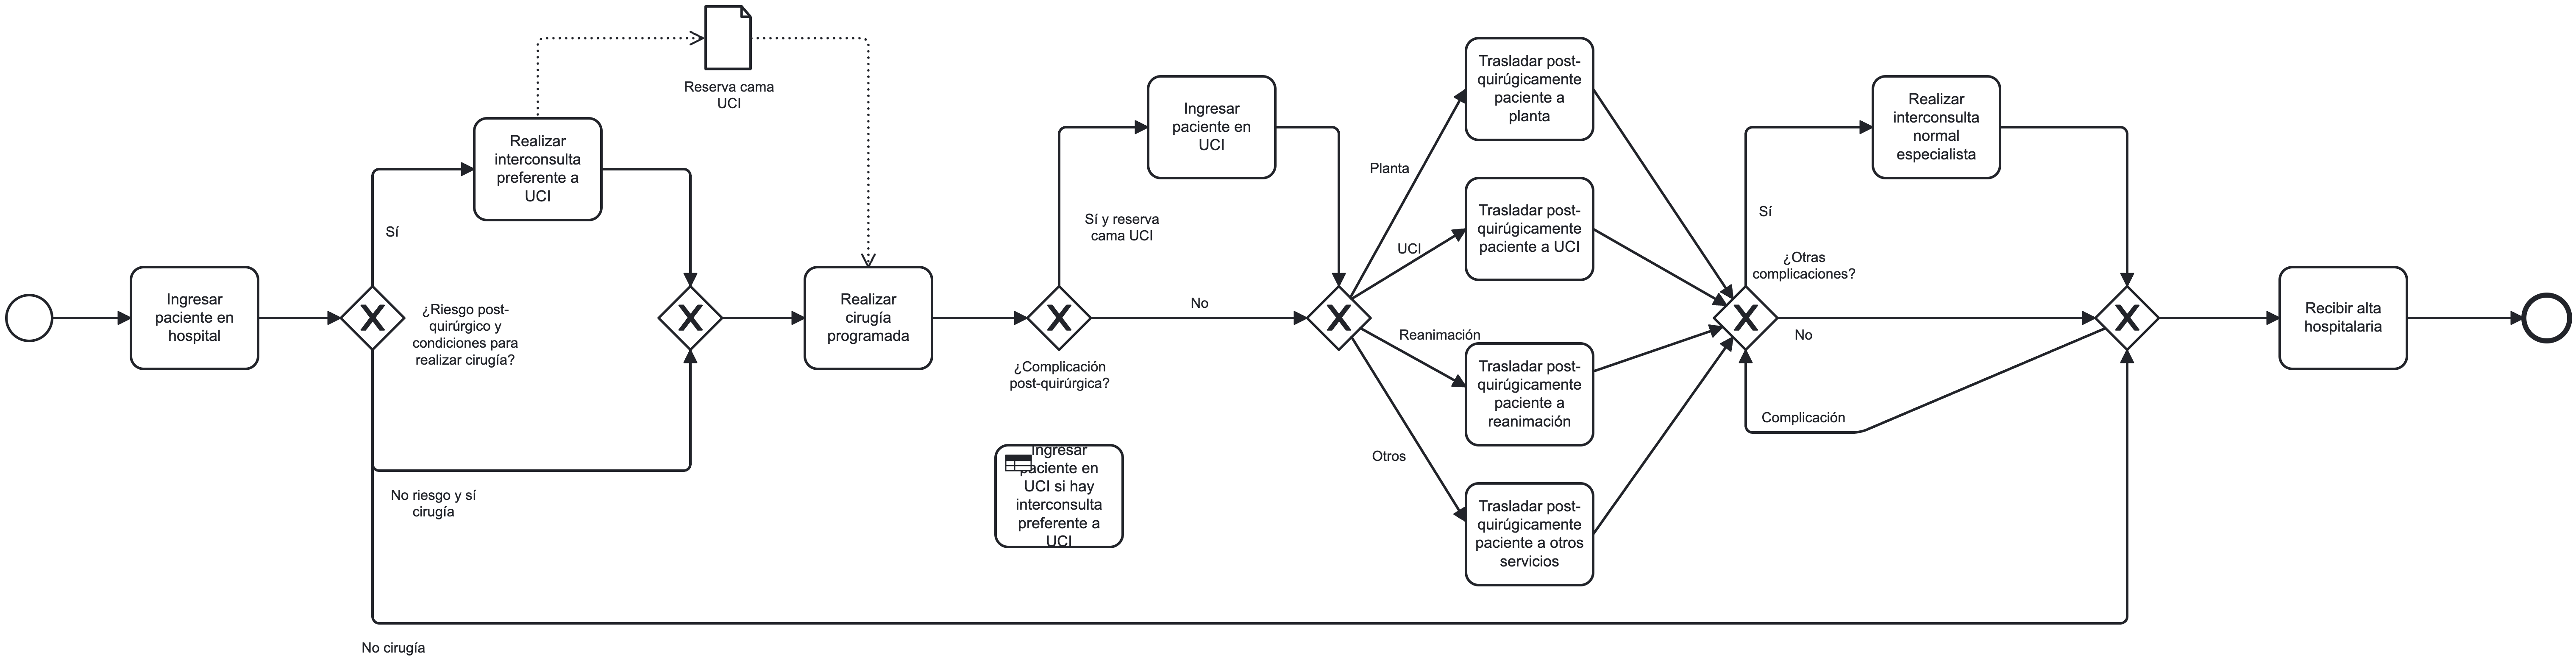
\includegraphics[width=\textheight]{bpmn_proceso_asistencial}
\caption{BPMN reference model of the elective surgical admission process (TO-BE model).}
\label{fig:bpmn}
\end{sidewaysfigure}

\section{Construction of the Event Log}
\label{sec:construccion}

This section describes how the event log was built from the tables of Section~\ref{sec:bd} for the population of Section~\ref{sec:poblacion}: the input and the definition of case and events, the ordering and cleaning of the events, the outputs produced, the two design decisions that shape the event log and the resulting event log.

\subsection{Input, Case and Events}

The event log was generated with a Python script (\code{build\_event\_log\_v3.py}). Its input is the export of the database to CSV files, one file per table with the same name as the table, produced from the PostgreSQL server with semicolon as separator and UTF-8 encoding. The script reads the four event tables of Table~\ref{tab:tablas} (\code{ftr\_hosp}, \code{ftr\_hosp\_interconsultas}, \code{ftr\_hosp\_int\_quirurgicas} and \code{ftr\_hosp\_traslados}), the coding table and the catalogs, and keeps only the episodes of the elective surgical branch.

The case is the hospitalization episode, identified by \code{id\_anonim\_episodio}. The patient code is kept as a case attribute, which allows grouping the episodes of the same patient. Each row of the four event tables is transformed into one or more events according to the rules in Table~\ref{tab:actividades}, which also gives the element of the reference model that each activity represents and the number of events obtained. The activity names are kept in Spanish, as they appear in the source database and in the code. The timestamp of each event is the date and time recorded in its source table. For \code{INGRESO}, \code{ALTA}, \code{EXITUS} and \code{TRASLADO\_OTRO\_HOSPITAL} it is the admission or discharge date. For the consultations it is the date of the consultation. For \code{QUIROFANO\_INICIO} and \code{QUIROFANO\_FIN} it is the start and the end of the intervention. For the \code{DESTINO\_*} activities it is also the end of the intervention, because the surgical table does not record a time of its own for the destination decision. For \code{INGRESO\_UCI} and \code{TRASLADO\_PLANTA} it is the start of the stay in the new bed.

\begin{table}[htbp]
\centering
\caption{Activities of the event log, their origin and their frequency.}
\label{tab:actividades}
\footnotesize
\begin{tabular}{L{4.5cm}L{3.9cm}L{3.6cm}r}
\toprule
Activity & Construction rule & BPMN element (Figure~\ref{fig:bpmn}) & Events \\
\midrule
\code{INGRESO} & Admission date from \code{ftr\_hosp} & Ingresar paciente en hospital & 1,475 \\
\code{INTERCONSULTA\_UCI} & Consultation with target service ICU & Realizar interconsulta preferente a UCI & 18 \\
\code{INTERCONSULTA\_ESPECIALISTA} & Consultation to any other service & Realizar interconsulta normal especialista & 452 \\
\code{QUIROFANO\_INICIO} / \code{FIN} & Start and end of each intervention & Realizar cirugía programada & 1,396 / 1,396 \\
\code{DESTINO\_PLANTA} & \code{codigo\_destino} ward or recovery room & Destination decision: Planta & 1,212 \\
\code{DESTINO\_UCI} & \code{codigo\_destino} ICU & Destination decision: UCI (bed reservation) & 124 \\
\code{DESTINO\_REANIMACION} & \code{codigo\_destino} post-anesthesia care unit & Destination decision: Reanimación & 53 \\
\code{DESTINO\_OTROS} & Home, day surgery unit, emergency care or others & Destination decision: Otros & 7 \\
\code{INGRESO\_UCI} & Actual transfer to the ICU (\code{ftr\_hosp\_traslados}) & Ingresar paciente en UCI & 148 \\
\code{TRASLADO\_PLANTA} & Actual transfer to another unit other than the ICU & Trasladar post-quirúrgicamente paciente a planta & 24 \\
\code{TRASLADO\_OTRO\_HOSPITAL} & Discharge reason: transfer & Not in the model & 1 \\
\code{EXITUS} & Discharge reason: death & Not in the model (discharge reason) & 9 \\
\code{ALTA} & Discharge date, remaining reasons & Recibir alta hospitalaria & 1,465 \\
\bottomrule
\end{tabular}
\end{table}

Two catalogs of the database intervene in the rules of Table~\ref{tab:actividades}: the anesthesia types and the postoperative destinations. Table~\ref{tab:catalogos} lists the codes of both catalogs, one block per catalog, and shows how each code is used: the anesthesia code becomes an attribute of the surgery, and the destination codes are grouped into the four \code{DESTINO\_*} activities. The ward and the recovery room are merged because the recovery room is a transit before the ward; the ICU and the post-anesthesia care unit are kept as destinations of their own; and the remaining destinations (home, day surgery unit, emergency care and others), which are rare, are grouped together.

\begin{table}[htbp]
\centering
\caption{Catalog codes used in the construction of the event log. The anesthesia codes feed a surgery attribute; the destination codes are grouped into the four \code{DESTINO\_*} activities.}
\label{tab:catalogos}
\small
\begin{tabular}{rL{6.0cm}L{5.2cm}}
\toprule
Code & Value & Use in the event log \\
\midrule
\multicolumn{3}{l}{Catalog \code{tipo\_anestesia\_pk} (anesthesia type)} \\
1 & Local & Surgery attribute (anesthesia) \\
2 & General & Surgery attribute (anesthesia) \\
4 & [Sin anestesia] (no anesthesia) & Surgery attribute (anesthesia) \\
5 & Regional & Surgery attribute (anesthesia) \\
6 & [Sin datos] (no data) & Surgery attribute (anesthesia) \\
7 & Gral-UCI (general, ICU destination) & Surgery attribute (anesthesia) \\
8 & Gral-REA (general, post-anesthesia care unit) & Surgery attribute (anesthesia) \\
9 & Sedaci\'on (sedation) & Surgery attribute (anesthesia) \\
\midrule
\multicolumn{3}{l}{Catalog \code{destinos\_postoperatorio\_quirofano} (postoperative destination)} \\
1 & PLANTA (ward) & Activity \code{DESTINO\_PLANTA} \\
2 & DESPERTAR (recovery room) & Activity \code{DESTINO\_PLANTA} \\
7 & UCI (ICU) & Activity \code{DESTINO\_UCI} \\
9 & REANIMACI\'ON (post-anesthesia care unit) & Activity \code{DESTINO\_REANIMACION} \\
3 & DOMICILIO (home) & Activity \code{DESTINO\_OTROS} \\
4 & UCSI (day surgery unit) & Activity \code{DESTINO\_OTROS} \\
5 & OTROS (others) & Activity \code{DESTINO\_OTROS} \\
8 & URGENCIAS (emergency care) & Activity \code{DESTINO\_OTROS} \\
\bottomrule
\end{tabular}
\end{table}

\subsection{Ordering and Cleaning of the Events}

Once the events were created, they were sorted within each case by timestamp. The timestamps of the database have a resolution of one minute, and therefore several events of the same case may share the same minute. This happens mainly at the end of the surgery: \code{QUIROFANO\_FIN} and the \code{DESTINO\_*} event take, by construction, the same timestamp, and in some cases the transfer to the ICU is recorded in the same minute. For these ties a fixed order was applied that reproduces the logic of the process: first the end of the surgery (\code{QUIROFANO\_FIN}), then the destination decision (\code{DESTINO\_*}) and then the actual admission to the ICU (\code{INGRESO\_UCI}). More generally, the tie-break follows the order admission, consultations, operating theater, destination, ICU, transfer and discharge. Without this rule, the order of two events in the same minute would depend on the order of the rows in the source files, and the same situation could produce different traces.

Then the events that fall outside the episode were discarded. An event was kept if its timestamp lies in the interval from one day before the admission date to one day after the discharge date, that is, in [\code{fecha\_ingreso} $-$ 1 day, \code{fecha\_alta} $+$ 1 day]. The one-day margin absorbs the acts recorded just before the admission (for example a preoperative consultation on the previous day) or just after the discharge. Only three events of the whole event log fell outside this interval: the start, the end and the destination of a single intervention whose recorded date is six years before its episode, which is a recording error.

\subsection{Outputs}

The script produces three outputs, each with a use of its own.

\begin{itemize}[leftmargin=*]
  \item \textbf{The event table}, in CSV and Parquet format (\code{eventlog\_pq.csv} and \code{.parquet}): one row per event, with the case, the activity, the timestamp, the attributes inherited from its source row (service, bed, priority, requesting and target service, type, category, approach and anesthesia of the intervention, postoperative destination, discharge reason) and the phase attribute (\code{fase} in the code) described below. This is the input of the PPM experiments of Chapter~\ref{cap:implementacion}, which read the Parquet file with pandas. The CSV copy allows inspecting the data with any tool.
  \item \textbf{The case table} (\code{eventlog\_pq\_casos.csv} and \code{.parquet}): one row per episode with the case attributes of Section~\ref{sec:atributos} and the candidate labels of Section~\ref{sec:etiquetas}. The experiments join it with the event table through the case code to obtain the static vector of each prefix and the label of each case.
  \item \textbf{The XES file} (\code{eventlog\_pq.xes.gz}), the standard format of PM, written with PM4Py. It contains the activities, the timestamps and the light attributes of each event, without missing text values, so that Disco, ProM and Celonis import it without errors. It is the input of the discovery and conformance checking of Section~\ref{sec:discovery}.
\end{itemize}

\subsection{Two Design Decisions}

Two design decisions deserve a detailed explanation, because they determine what the event log can say about the planning of the process and about what actually happened.

The first decision is the \textbf{distinction between planned destination and actual transfer}. The surgical table records, at the end of the operation, the postoperative destination decided by the surgical team: the ward, the ICU, the post-anesthesia care unit or another unit. It is a decision, not a movement, and the table does not even store a time for it. The transfers table, on the other hand, records the physical movement of the patient from one bed to another, with the time at which the new bed was occupied. The two are different and the event log keeps them as different activities: \code{DESTINO\_*} for the decision, with the timestamp of the end of the surgery, and \code{INGRESO\_UCI} or \code{TRASLADO\_PLANTA} for the movement, with its actual time. Version 2 of the event log did not have the \code{DESTINO\_*} activities and recorded only the movements; the decision was visible only as an attribute of the surgery event. Making the decision an activity of its own is what allows comparing, in Section~\ref{sec:destino_uci}, what was planned with what happened. The actual times are kept even when they contradict the expected order: in 34 cases the transfer to the ICU is recorded before the end of the surgery, because the bed in the ICU is assigned while the patient is still in the operating theater. These cases were not corrected, since altering the times would hide a feature of the recording system that conformance checking must detect.

The second decision is the \textbf{phase attribute} (\code{fase} in the code). Each event is labeled with the phase of the episode in which it occurs, computed with respect to the first \code{QUIROFANO\_INICIO} of the case. An event is \emph{preoperative} if it precedes it, \emph{surgery} if it is the start or the end of an intervention, \emph{postoperative} if it follows the first surgery and \emph{without surgery} if the case has no recorded intervention. The event log has 1,472 preoperative, 4,188 surgery, 1,769 postoperative and 351 without-surgery events. This attribute has two uses. In the construction of the prefixes (Section~\ref{sec:prefijos}) it indicates whether the surgery is already in the prefix, and therefore whether the surgery attributes may be used. In the definition of the labels it separates, for example, the ICU consultations before and after the surgery, or the postoperative complication from the preoperative events.

\subsection{The Resulting Event Log}

Table~\ref{tab:resumen_log} summarizes the event log obtained. The dominant variant, \code{INGRESO} $\rightarrow$ \code{QUIROFANO\_INICIO} $\rightarrow$ \code{QUIROFANO\_FIN} $\rightarrow$ \code{DESTINO\_PLANTA} $\rightarrow$ \code{ALTA}, covers 916 cases (62\%). It is followed by the variants with a specialist consultation before, during or after the surgery (186 cases), the admission without recorded surgery (100 of the 142 episodes without a recorded intervention go directly from \code{INGRESO} to \code{ALTA}; the rest have consultations or transfers), the exit to the post-anesthesia care unit (44) and the planned ICU (36). Some episodes have more than one transfer to the ICU, which is why Table~\ref{tab:actividades} counts 148 \code{INGRESO\_UCI} events for the 131 episodes with an ICU admission. Figure~\ref{fig:dfg} shows the complete DFG of the elective surgical process obtained with PM4Py, and Figure~\ref{fig:disco} the frequency map of the same event log in Disco, which draws the same 14 activities and the same transitions with the frequency of each one.

\begin{table}[htbp]
\centering
\caption{Summary of the event log (version 3).}
\label{tab:resumen_log}
\small
\begin{tabular}{L{8cm}r}
\toprule
Measure & Value \\
\midrule
Cases (episodes) & 1,475 \\
Patients & 1,308 \\
Events & 7,780 \\
Activities & 14 \\
Variants & 97 \\
Directly-follows transitions & 59 \\
Events per case: median (minimum, maximum) & 5 (2, 32) \\
Cases with recorded surgery & 1,333 (90.4\%) \\
Cases with more than one intervention & 46 \\
Length of stay in days: median (mean, maximum) & 3.2 (4.9, 195) \\
Admission dates & 1 March 2023 to 29 February 2024 \\
\bottomrule
\end{tabular}
\end{table}

\begin{figure}[htbp]
\centering
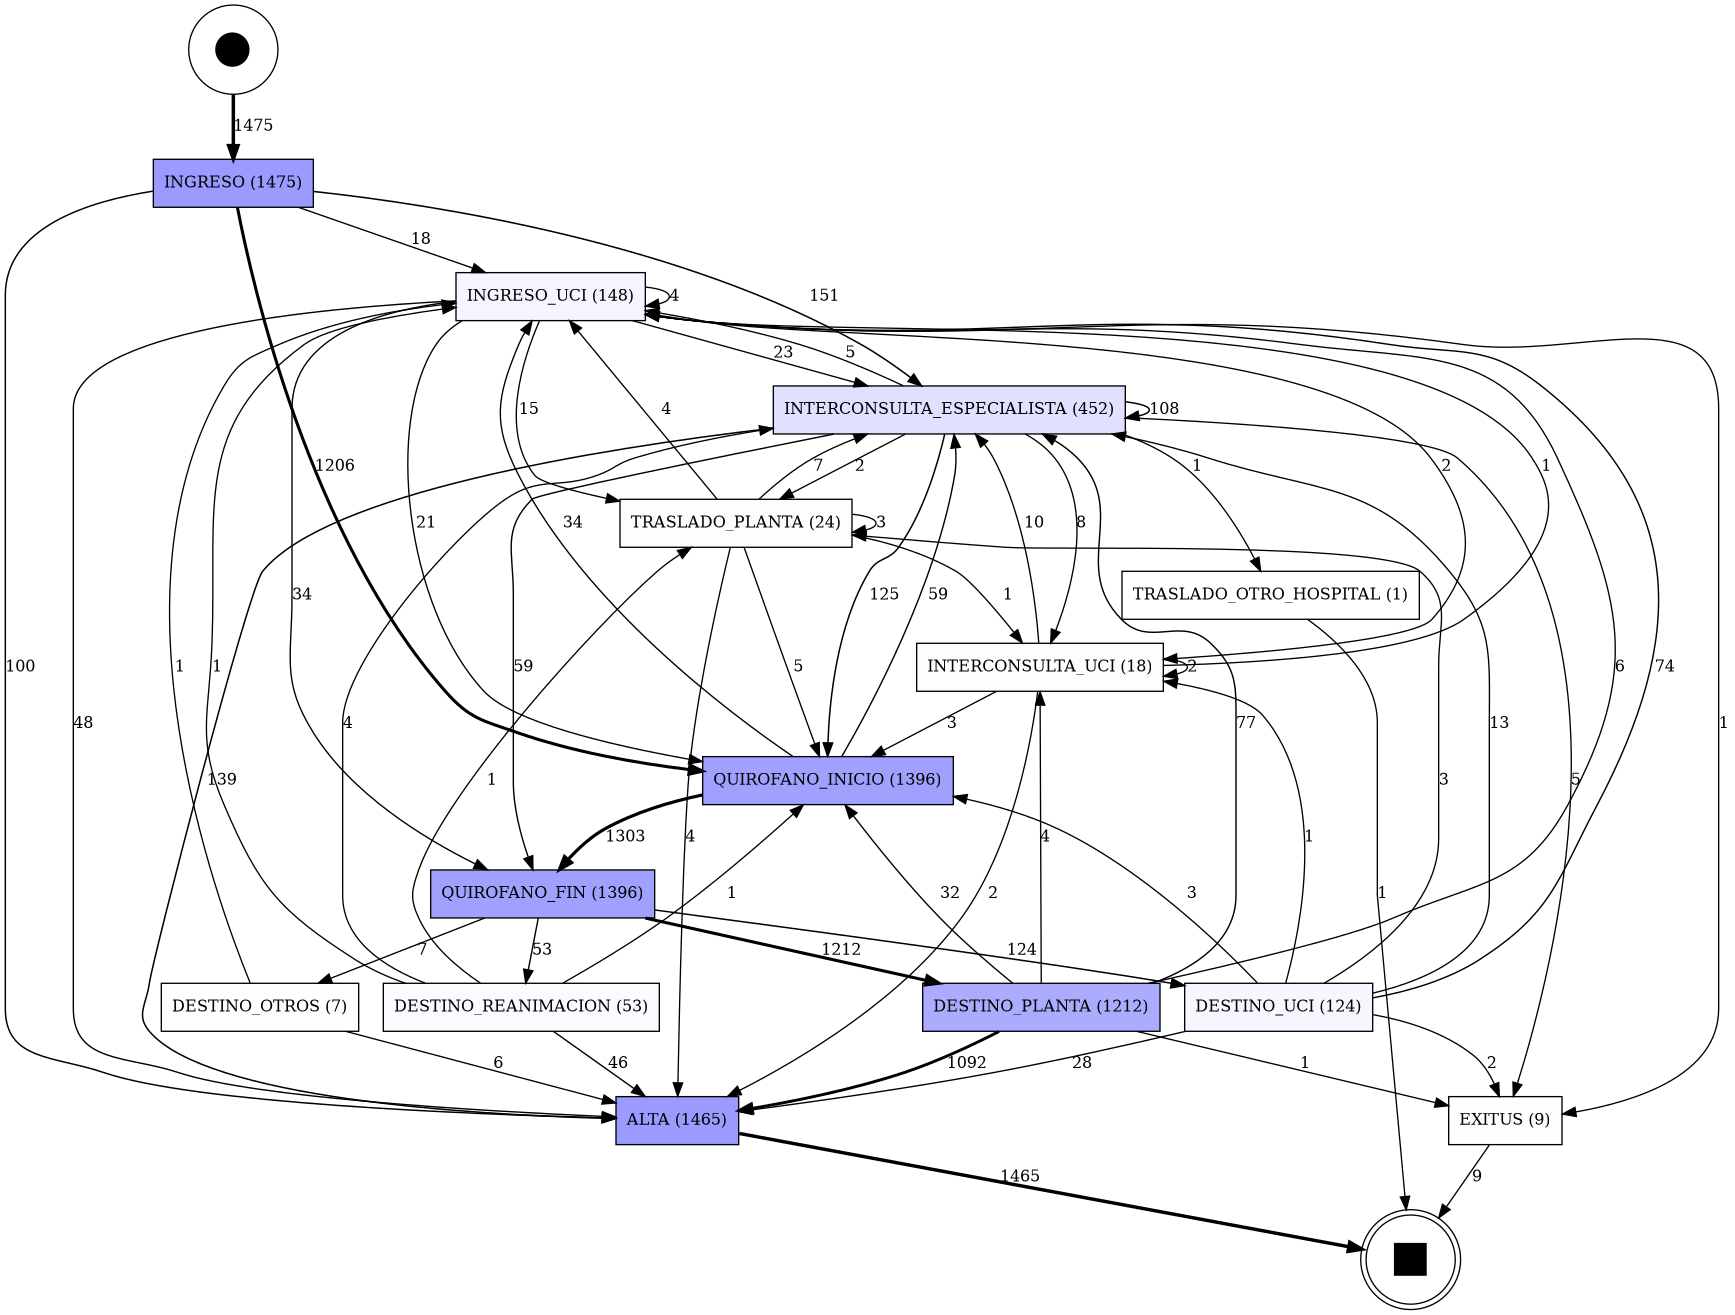
\includegraphics[width=0.85\textwidth]{dfg_v3}
\caption{DFG of the elective surgical process (PM4Py), with the frequency of each activity and of each transition.}
\label{fig:dfg}
\end{figure}

\begin{figure}[htbp]
\centering
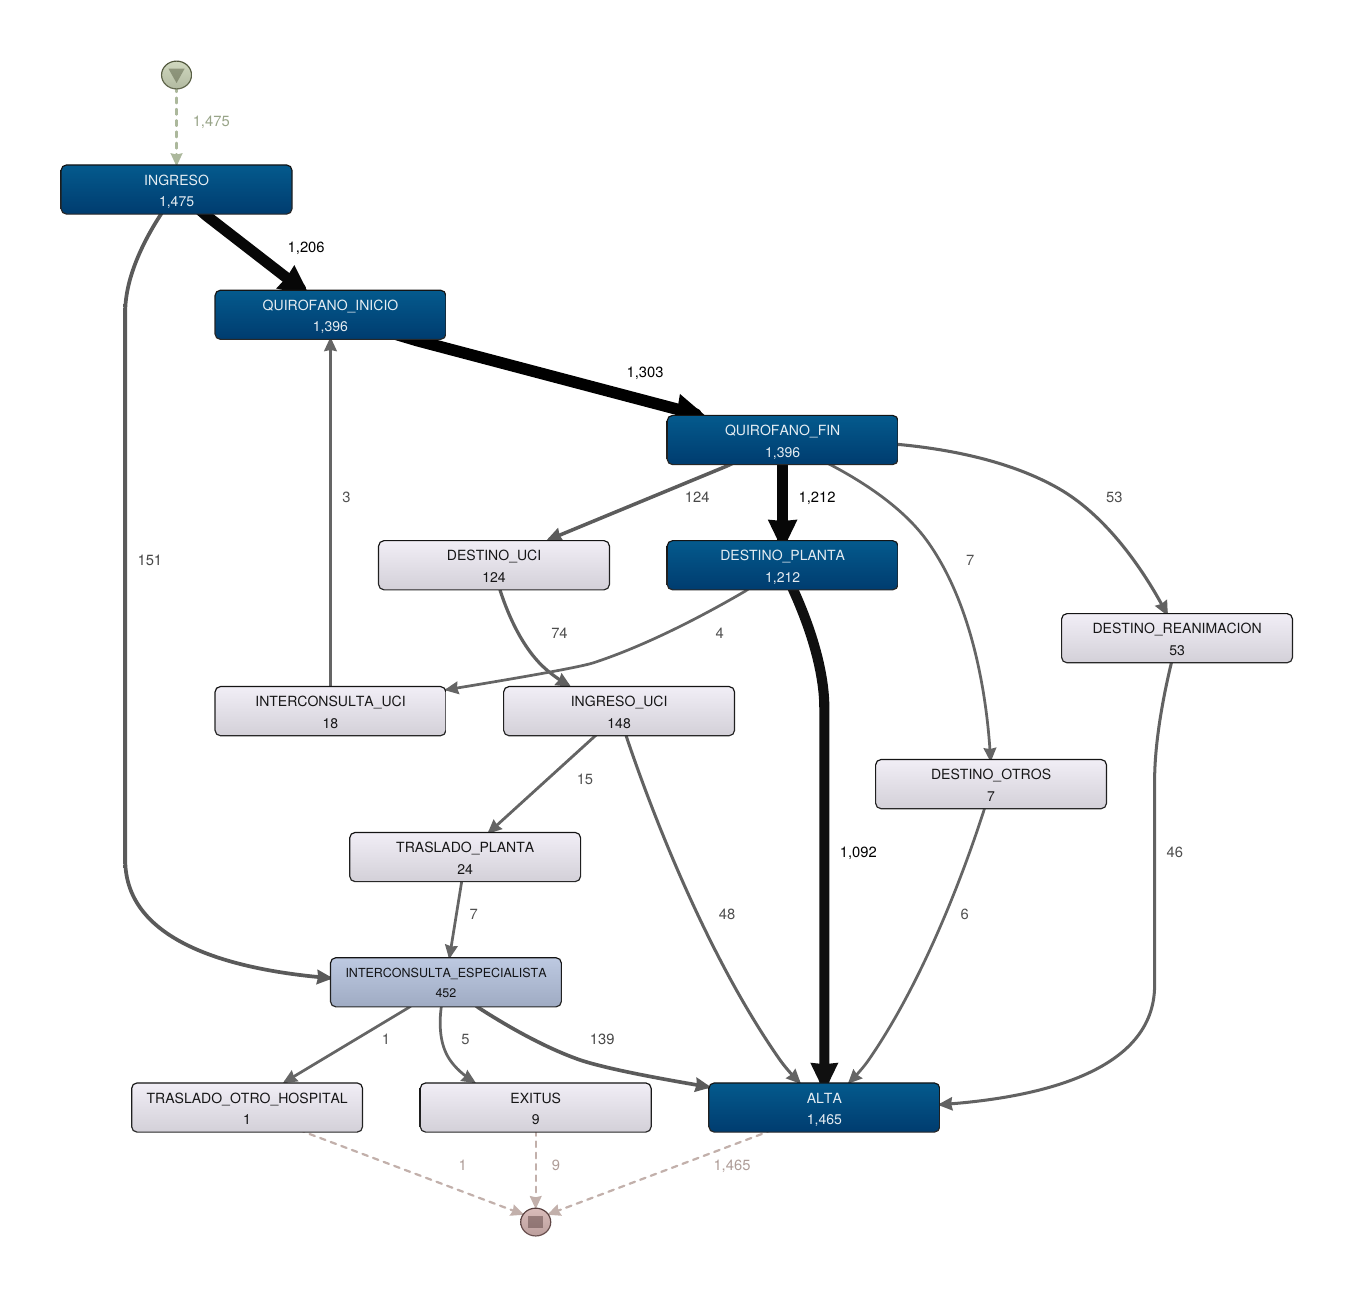
\includegraphics[width=0.95\textwidth]{disco_frecuencia}
\caption{Frequency map of the event log in Disco.}
\label{fig:disco}
\end{figure}

\section{Candidate Outcome Labels}
\label{sec:etiquetas}

The first thing predicted in this work is the \textbf{next activity} of a running case (Prediction~1). This prediction needs no label: the target of each prefix is the activity that follows it in the trace, and it is the prediction addressed by the Entropy-Driven Next Activity Prediction Approach of Zare et al.\ \cite{zare2025}, with which this work is compared.

The outcome-based predictions (Predictions~2 and~3) do need a label per case, and here the work meets a limitation of the data. FTR, as defined in Section~\ref{sec:datos_clinicos}, is the death after a complication that could have been treated. The database does not record whether a complication occurred, whether it was detected or whether the response was adequate. Therefore FTR cannot be labeled directly. What can be done is to define \textbf{candidate labels} from the observable precursors of FTR that the data do record: the admission to the ICU, the prolonged length of stay, the consultations, the death and the transfer to another hospital. Ten binary labels were defined from the case table. Table~\ref{tab:etiquetas} lists them with their number of positive cases and the assessment of their feasibility as a prediction target. The feasibility criterion is the number of positives available for evaluation: with a temporal split in which the 20\% most recent cases form the test set (295 cases), a label with 1\% of positives leaves three positive cases in the test set, which is not enough to measure anything.

\begin{table}[htbp]
\centering
\caption{Candidate outcome labels and their feasibility.}
\label{tab:etiquetas}
\small
\begin{tabular}{L{4.6cm}L{4.6cm}L{1.9cm}L{2.5cm}}
\toprule
Label & Definition & Positives & Feasibility \\
\midrule
\code{label\_ingreso\_uci} & Any \code{INGRESO\_UCI} in the episode & 131 (8.9\%) & Feasible (Prediction~2) \\
\code{label\_estancia\_prolongada} & Length of stay above the 90th percentile (8.74 days) & 148 (10.0\%) & Feasible (Prediction~3) \\
\code{label\_complicacion\_postop} & Postoperative ICU, postoperative specialist consultation, death or transfer & 240 (16.3\%) & Complementary \\
\code{label\_uci\_no\_planificada} & \code{INGRESO\_UCI} without postoperative destination ICU & 21 (1.4\%) & Complementary, with cross-validation \\
\code{label\_ftr\_compuesto} & Death, ICU admission or transfer & 135 (9.2\%) & Redundant with Prediction~2 (131 of 135) \\
\code{label\_reingreso\_7d} & Readmission within 7 days & 23 (1.6\%) & Unfeasible \\
\code{label\_exitus\_intrahosp} & In-hospital death & 9 (0.6\%) & Unfeasible \\
\code{label\_exitus\_30d} / \code{90d} & Death within 30 / 90 days & 10 / 26 & Unfeasible \\
\code{label\_traslado\_otro\_hosp} & Transfer to another hospital & 1 & Unfeasible \\
\bottomrule
\end{tabular}
\end{table}

The labels are read as follows.

\begin{itemize}[leftmargin=*]
  \item \textbf{ICU admission} (\code{label\_ingreso\_uci}) is positive when the episode has at least one actual transfer to the ICU, whatever its moment and whether or not it was planned. With 131 positives (8.9\%) it is feasible and it is the label of \textbf{Prediction~2}. Its relation with the planning of the surgery is analyzed in Section~\ref{sec:destino_uci}.
  \item \textbf{Prolonged length of stay} (\code{label\_estancia\_prolongada}) is positive when the stay exceeds the 90th percentile of the population, 8.74 days. The threshold is a percentile, and not a clinical value, because the expected length of stay depends on the surgery. With 148 positives (10.0\%) it is feasible and it is the label of \textbf{Prediction~3}.
  \item \textbf{Postoperative complication} (\code{label\_complicacion\_postop}) is a broad label: it is positive when, after the surgery, there is an ICU admission, a consultation to a specialist, a death or a transfer. It has the most positives (240, 16.3\%), but it mixes very different situations, from a routine consultation to a death. It is studied as a complementary analysis.
  \item \textbf{Unplanned ICU admission} (\code{label\_uci\_no\_planificada}) is positive when there is an ICU admission and the postoperative destination recorded in the operating theater was not the ICU. It is the label closest to FTR, because it captures the complication that nobody anticipated, but it has only 21 positives (1.4\%). It is studied as a complementary analysis with cross-validation instead of a temporal split, so that no positive case is lost to the split.
  \item \textbf{Composite FTR} (\code{label\_ftr\_compuesto}), positive on death, ICU admission or transfer, is redundant with ICU admission: 131 of its 135 positives are ICU admissions. It is not studied separately.
  \item \textbf{Readmission within 7 days}, \textbf{in-hospital death}, \textbf{death within 30 or 90 days} (computed from \code{fecha\_exitus}) and \textbf{transfer to another hospital} have between 1 and 26 positives. They are unfeasible as prediction targets. Death, the most serious outcome of FTR, is almost nonexistent in elective surgery (0.6\%), which rules out any mortality-based target.
\end{itemize}

In summary, ICU admission and prolonged length of stay are the only outcomes with enough positives for an evaluation with a temporal split. Postoperative complication has even more positives but is heterogeneous, and unplanned ICU admission, the purest clinical target, has only 21 cases.

\section{Planned Destination versus Actual ICU Admission}
\label{sec:destino_uci}

Before predicting the ICU admission, it was checked how it relates to the destination decided in the operating theater. The result, shown in Table~\ref{tab:destino_uci}, is the finding that most conditions the work. The table crosses the postoperative destination recorded for the first intervention of each episode with the actual ICU admission. Of the 110 cases with planned destination ICU, \textbf{all 110 are admitted to the ICU}: the ICU destination is, in practice, the bed reservation. Of the 1,165 cases with destination ward, only 11 end up in the ICU; of the 52 with destination post-anesthesia care unit, two. The \textbf{21 ICU admissions without a planned ICU destination} (11 + 2 + 1 + 7 without surgery) are the \emph{unplanned} ICU admissions, the complication that nobody anticipated: FTR in the strict sense.

\begin{table}[htbp]
\centering
\caption{Planned postoperative destination (first intervention) versus actual ICU admission.}
\label{tab:destino_uci}
\begin{tabular}{lrr}
\toprule
Planned destination & Cases & Admitted to the ICU \\
\midrule
Ward (ward + recovery room) & 1,165 & 11 \\
ICU & 110 & 110 (100\%) \\
Post-anesthesia care unit & 52 & 2 \\
Others (day surgery unit) & 6 & 1 \\
No surgery / no data & 142 & 7 \\
\midrule
\textbf{Total} & \textbf{1,475} & \textbf{131} \\
\bottomrule
\end{tabular}
\end{table}

Two consequences follow from this table. The first affects the reading of the reference model: the `priority consultation to the ICU' that the BPMN model places before the surgery does not exist before the surgery in the data (zero preoperative cases; the 18 ICU consultations recorded are postoperative). The bed reservation of the model materializes in the data as the postoperative destination recorded in the operating theater, and this is how it is read in the conformance checking of Chapter~\ref{cap:implementacion}. The second affects prediction: any model that sees \code{DESTINO\_UCI} in the prefix predicts the ICU admission trivially, because it is reading a decision already taken. Measuring real predictive ability therefore requires hiding that information or changing the target.

This single table gives rise to three ways of asking the question `will the patient be admitted to the ICU?', which differ in the information available to the model and in the population. Figure~\ref{fig:variantes} summarizes them.

\begin{itemize}[leftmargin=*]
  \item \textbf{Variant A: without planning information}. The population is the whole event log (1,475 cases) and the label is the ICU admission (131 positives). The planned destination is removed from the prefixes, and the anesthesia that reveals it (\code{Gral-UCI}, general anesthesia with ICU destination, recorded at the start of the surgery) is recoded as plain general anesthesia. The model must predict the admission with what the patient, the service and the surgery say. This is \textbf{Prediction~2}, the one reported in Chapter~\ref{cap:implementacion} as the main result, because it measures what a model could add to the decision of the surgical team.
  \item \textbf{Variant B: with planning information}. Same population and same label, but the destination and the anesthesia stay in the prefix. The model only has to read them. The result is not a prediction but an \textbf{upper bound}: it measures how much of the ICU admission is already decided in the operating theater, and it serves as a reference for the other two variants.
  \item \textbf{Variant C: unplanned ICU admission}. The population is restricted to the 1,365 cases without a planned ICU destination and the label is the unplanned admission (21 positives). Here the destination is legitimate information, because no positive case has the ICU as destination, and therefore nothing has to be hidden. It is the purest clinical question, but with only 21 positives it is evaluated as a complementary analysis.
\end{itemize}

\begin{figure}[htbp]
\centering
\begin{tikzpicture}[
  ev/.style={draw=black!60, fill=black!5, rounded corners=2pt, font=\tiny\ttfamily, minimum height=4.5mm, inner sep=2.5pt},
  hid/.style={ev, draw=red!70, fill=red!8, text=red!70!black},
  rec/.style={ev, draw=orange!80!black, fill=yellow!25},
  lab/.style={font=\footnotesize, anchor=east, align=right, text width=3.3cm},
  note/.style={font=\scriptsize, anchor=north west, text width=9.2cm, align=left}]
\node[lab] at (-0.2,3.7) {\textbf{A}: Prediction~2\\ 1,475 cases, 131 positives};
\node[ev, anchor=west] (a1) at (0,3.7) {INGRESO};
\node[ev, right=1.5mm of a1] (a2) {QUIROFANO\_INICIO};
\node[rec, right=1.5mm of a2] (a3) {Gral-UCI $\to$ General};
\node[ev, right=1.5mm of a3] (a4) {QUIROFANO\_FIN};
\node[hid, right=1.5mm of a4] (a5) {DESTINO\_UCI};
\node[note] at (0,3.4) {Planning information hidden: the destination is removed and the anesthesia recoded. The model predicts.};
\node[lab] at (-0.2,2.05) {\textbf{B}: upper bound\\ 1,475 cases, 131 positives};
\node[ev, anchor=west] (b1) at (0,2.05) {INGRESO};
\node[ev, right=1.5mm of b1] (b2) {QUIROFANO\_INICIO};
\node[ev, right=1.5mm of b2] (b3) {Gral-UCI};
\node[ev, right=1.5mm of b3] (b4) {QUIROFANO\_FIN};
\node[ev, right=1.5mm of b4] (b5) {DESTINO\_UCI};
\node[note] at (0,1.75) {Planning information visible: the model reads the decision already taken.};
\node[lab] at (-0.2,0.4) {\textbf{C}: unplanned ICU\\ 1,365 cases, 21 positives};
\node[ev, anchor=west] (c1) at (0,0.4) {INGRESO};
\node[ev, right=1.5mm of c1] (c2) {QUIROFANO\_INICIO};
\node[ev, right=1.5mm of c2] (c3) {Gral-REA};
\node[ev, right=1.5mm of c3] (c4) {QUIROFANO\_FIN};
\node[ev, right=1.5mm of c4] (c5) {DESTINO\_PLANTA};
\node[note] at (0,0.1) {Cases with planned destination ICU excluded: no positive has it, and therefore nothing has to be hidden.};
\end{tikzpicture}
\caption{The three variants of the ICU admission question. Each row shows a prefix as the model sees it: the red element is removed from the prefix and the yellow one is recoded.}
\label{fig:variantes}
\end{figure}

Chapter~\ref{cap:implementacion} evaluates the three variants with the same models and the same protocol: variant A as Prediction~2 (Section~\ref{sec:pred2}) and variants B and C as complementary analyses (Sections~\ref{sec:compl_b} and~\ref{sec:compl_c}). Figure~\ref{fig:niveles_abc} in that chapter gives the detail of the implementation of each one.

\section{Warnings About Information Leakage}
\label{sec:fugas}

Information leakage occurs when a model uses, as input, information that would not be available at the moment of the prediction, or that is a consequence of the outcome to be predicted. The planned destination of the previous section is the clearest case. In addition, the following variables of the case table were identified as leakage and excluded from the models.

\begin{itemize}[leftmargin=*]
  \item \textbf{Discharge service} (\code{servicio\_alta}) and \textbf{discharge reason} (\code{motivo\_alta}). They are known at discharge. The reason reveals death and transfer directly, and the service reveals whether the patient was in the ICU at the end.
  \item \textbf{Length of stay} (\code{estancia\_dias}), the difference between the discharge and admission dates. It is the variable from which the label of Prediction~3 is derived, and it is also longer in the cases with ICU admission.
  \item \textbf{Number of events} of the case (\code{n\_eventos}) and \textbf{bed at discharge} (\code{cama\_al\_alta}). The number of events is only known when the case ends and it grows with the complications; the bed at discharge identifies the unit in which the patient ended.
  \item \textbf{Number of coded diagnoses} (\code{n\_diag}), the less obvious one. ICD-10 coding is performed at discharge by the coding unit, which reviews the whole episode and records one diagnosis per condition treated. Complications add diagnoses: the cases with unplanned ICU admission have 11.5 diagnoses on average versus 5.9 for the rest. The variable looks like a comorbidity measure available at admission, but it is in fact a summary of what happened. As shown in Section~\ref{sec:sens_ndiag}, including \code{n\_diag} doubles the apparent performance on the scarcest target, an unmistakable symptom of leakage.
\end{itemize}

The \textbf{ICD chapter of the main diagnosis} (\code{cie\_capitulo}) comes from the same coding, but it is kept with reservations, because in elective surgery the main diagnosis is the condition for which the surgery was scheduled, and it is known at admission.

\section{Process Entropy}
\label{sec:entropia}

The entropy of the event log was computed with the definition of the Entropy-Driven Next Activity Prediction Approach \cite{zare2025}, introduced in Section~\ref{sec:zare}. The computation has three steps. First, every pair of consecutive events of each trace is counted as one directly-follows transition $a \rightarrow b$. The 1,475 traces of the event log produce 6,305 transitions of 59 distinct types. Second, the probability of each transition type is its relative frequency: for example, the most frequent one, \code{QUIROFANO\_INICIO} $\rightarrow$ \code{QUIROFANO\_FIN}, appears 1,303 times, and therefore $p = 1{,}303 / 6{,}305 = 0.207$. Third, the Shannon entropy of this distribution is computed as $H = -\sum_t p(t)\log_2 p(t)$. The four dominant transitions (surgery start to end, surgery end to ward destination, admission to surgery and ward destination to discharge, each with $p$ between 0.17 and 0.21) contribute 1.82 bits, and the other 55 transitions, 27 of them with five occurrences or fewer, contribute 1.57 bits. The total is \textbf{3.39 bits} (3.54 bits if the artificial start and end markers of each trace are included, which adds four transition types).

Version 2 of the event log, the one without the destination activities (Section~\ref{sec:historia_tablas}), had 3.04 bits. Adding the postoperative destination contributes about 0.35 bits, because the operating theater comes to have four exits instead of one. The event log falls in the medium band of the paper, between BPIC 2017 (3.24) and BPIC 2020 Prepaid Travel Cost (3.64), the band in which, according to the authors, classical models should perform close to deep ones. Figure~\ref{fig:entropia} places both versions of the event log on the scale of the paper. This prediction is contrasted with the results of the next chapter.

\begin{figure}[htbp]
\centering
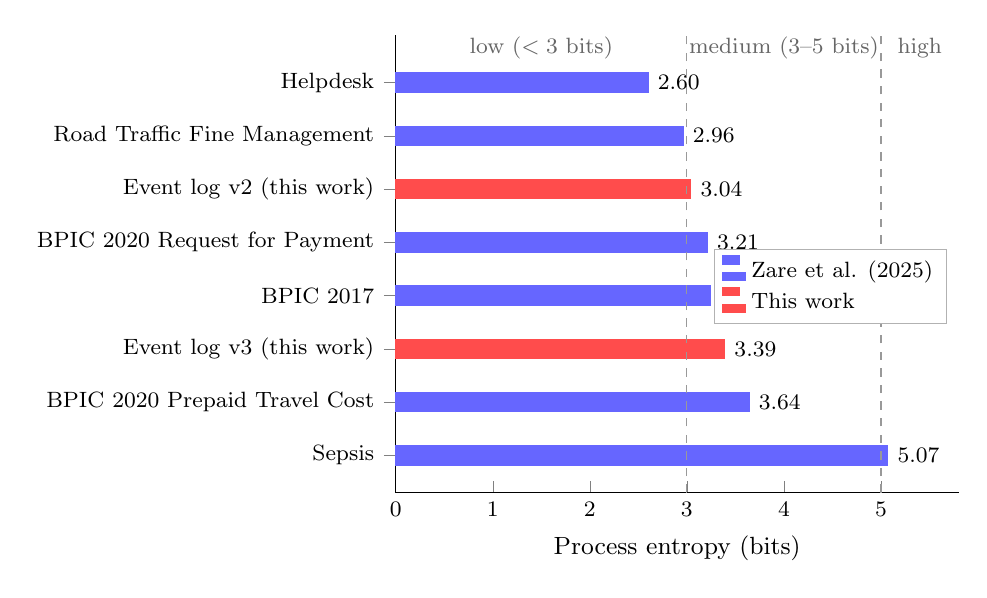
\begin{tikzpicture}
\begin{axis}[
  xbar, bar shift=0pt, width=0.72\textwidth, height=7.4cm, bar width=7pt,
  xmin=0, xmax=5.8, ymin=-0.7, ymax=7.9,
  xlabel={Process entropy (bits)}, xlabel style={font=\small},
  ytick={0,1,2,3,4,5,6,7},
  yticklabels={Sepsis, BPIC 2020 Prepaid Travel Cost, Event log v3 (this work), BPIC 2017, BPIC 2020 Request for Payment, Event log v2 (this work), Road Traffic Fine Management, Helpdesk},
  yticklabel style={font=\footnotesize}, tick label style={font=\footnotesize},
  nodes near coords, nodes near coords style={font=\footnotesize, /pgf/number format/fixed, /pgf/number format/precision=2, /pgf/number format/fixed zerofill},
  axis x line*=bottom, axis y line*=left, clip=false,
  legend style={at={(0.98,0.45)}, anchor=east, font=\footnotesize, draw=black!30}, legend cell align=left]
\addplot[fill=blue!60, draw=blue!60] coordinates {(2.60,7) (2.96,6) (3.21,4) (3.24,3) (3.64,1) (5.07,0)};
\addplot[fill=red!70, draw=red!70] coordinates {(3.04,5) (3.39,2)};
\legend{Zare et al. (2025), This work}
\draw[black!40, dashed] (axis cs:3,-0.7) -- (axis cs:3,7.9);
\draw[black!40, dashed] (axis cs:5,-0.7) -- (axis cs:5,7.9);
\node[font=\footnotesize, black!60] at (axis cs:1.5,7.65) {low ($< 3$ bits)};
\node[font=\footnotesize, black!60] at (axis cs:4.0,7.65) {medium (3--5 bits)};
\node[font=\footnotesize, black!60] at (axis cs:5.4,7.65) {high};
\end{axis}
\end{tikzpicture}
\caption[Process entropy of the two versions of the event log compared with the six event logs of the Entropy-Driven Next Activity Prediction Approach.]{Process entropy of the two versions of the event log of this work compared with the six event logs evaluated in the Entropy-Driven Next Activity Prediction Approach \cite{zare2025}; the dashed lines separate the low, medium and high entropy bands of the paper.}
\label{fig:entropia}
\end{figure}
